\section{IDN data format}\label{sec:idn-data-format}

The IDN file starts with \texttt{IDENCOMP} bytes encoded in ASCII, followed
by the version number (currently always 1).
Then, there is the metadata section, which contains the number of metadata
items and the items themselves.
Currently, only one type of metadata item is supported: model identifiers,
which indicate which models a file uses, to allow the decompressor to load
the corresponding models (or throw an error if they are unavailable).

The file header is followed by an arbitrary number of data blocks.
The data block header consists of the compressed data length and
CRC32\cite{rfc3385} checksum of all the sequence data in a block.
Then, it is followed by an arbitrary number of slices.

Each slice is either a ``switch model'' slice that instructs the decompressor
to use a specific model for the subsequent sequences or a ``sequence'' slice,
which is a compressed sequence data.
For completeness, the sequence identifiers (names) may also appear in a file
as a separate slice, containing all of the sequence names separated by
newlines, and compressed using either Deflate (for lower compression quality
options) or Brotli (for higher).

\begin{figure}[!ht]
    \centering
    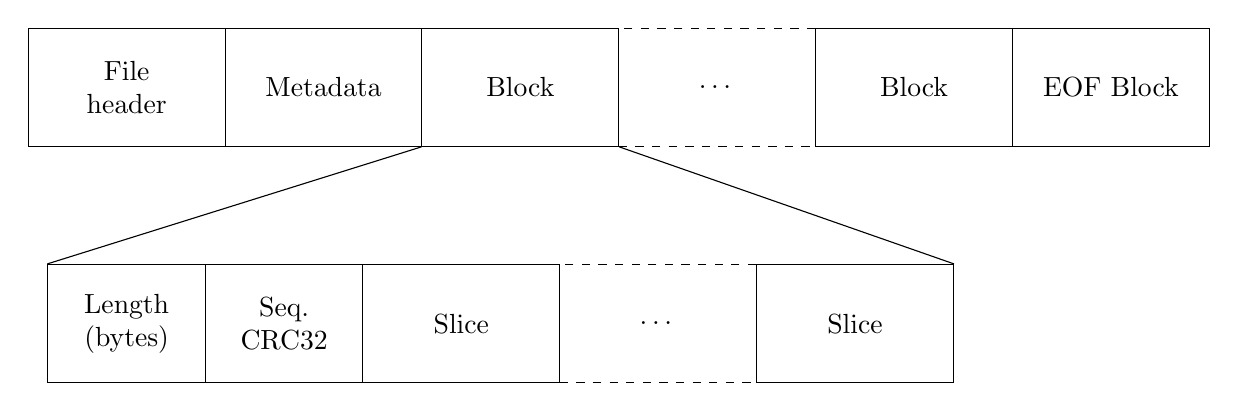
\begin{tikzpicture}[transform shape]
    \node at (0,3) [minimum height=1.5cm,minimum width=2.5cm,draw,align=center] (header) {File\\header};
    \node at (2.5,3) [minimum height=1.5cm,minimum width=2.5cm,draw] (metadata) {Metadata};
    \node at (5,3) [minimum size=1.5cm,minimum width=2.5cm,draw] (b1) {Block};
    \node at (7.5,3) [minimum height=1.5cm,minimum width=2.5cm,style=dashed,draw,inner sep=0] (b2) {\ldots};
    \node at (10,3) [minimum height=1.5cm,minimum width=2.5cm,draw] (b3) {Block};
    \node at (12.5,3) [minimum size=1.5cm,minimum width=2.5cm,draw] (beof) {EOF Block};

    \node at (0,0) [minimum height=1.5cm,minimum width=2cm,draw,align=center] (b_length) {Length\\(bytes)};
    \node at (2,0) [minimum height=1.5cm,minimum width=2cm,draw,align=center] (b_checksum) {Seq.\\CRC32};
    \node at (4.25,0) [minimum height=1.5cm,minimum width=2.5cm,draw] (slice1) {Slice};
    \node at (6.75,0) [minimum height=1.5cm,minimum width=2.5cm,style=dashed,draw,inner sep=0] (slice2) {\ldots};
    \node at (9.25,0) [minimum size=1.5cm,minimum width=2.5cm,draw] (slice3) {Slice};

    \draw (b1.south west) -- (b_length.north west);
    \draw (b1.south east) -- (slice3.north east);
\end{tikzpicture}

    \caption{%
        High-level diagram of the IDN file format
    }
    \label{fig:idn-file-format}
\end{figure}
